\section{Laboratório de Operações e Processos}
	O Laboratório de Operações e Processos (LOP) é um dos diversos laboratórios para fins de ensino e pesquisa pertencentes ao Departamento de Engenharia Química da UFMG (DEQ). Ainda existem outros laboratórios vinculados ao departamento cuja finalidade é prestar serviços às comunidades interna e externa à UFMG \footnote{\url{http://www.deq.ufmg.br/departamento/infraestrutura}}.
	
	O LOP possui quatro plantas didáticas: \textbf{explicar aqui brevemente as 4 plantas constituintes do laboratório}
	
	%explicar aqui agora sobre a planta de trocador existente
	O trocador de calor existente no laboratório, cuja imagem pode ser vista na figura~\ref{img1}, é do tipo \textcolor{red}{tubular}. 
	
	\begin{figure}[!htb]
		\centering
		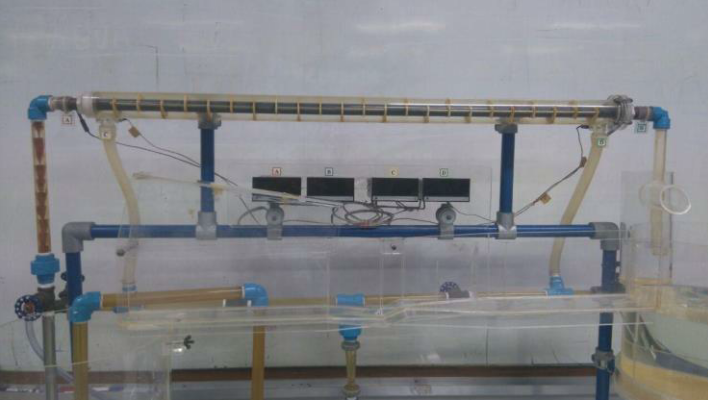
\includegraphics{img1}  %pode alterar o tamanho
		\caption{Trocador de Calor presente no LOP.}
		\label{img1}
	\end{figure}

	Este trocador de calor foi instalado no laboratório em \textcolor{red}{colocar aqui a história do trocador de calor} e originalmente possuía apenas a indicação das medidas de temperatura. A imagem \textcolor{red}{(colocar a referência)} destaca os sensores de temperatura instalados inicialmente. A medição de vazão era inferida através da utilização de uma Calha Parshall\footnote{\url{http://www.dec.ufcg.edu.br/saneamento/PARSHALL.html}}.
		
	Posteriormente, em 2016 um projeto de modernização desta planta foi iniciado por \cite{luiz2016}.  O projeto consistiu na implementação de um sistema embarcado para monitoramento, operação e controle da planta. Para alcançar o objetivo, sensores 